
%(BEGIN_QUESTION)
% Copyright 2009, Tony R. Kuphaldt, released under the Creative Commons Attribution License (v 1.0)
% This means you may do almost anything with this work of mine, so long as you give me proper credit

Read and outline the ``Interface Problems'' subsection of the ``Level Gauges (Sightglasses)'' section of the ``Continuous Level Measurement'' chapter in your {\it Lessons In Industrial Instrumentation} textbook relevant to {\it liquid-liquid interface measurement}.  Note the page numbers where important illustrations, photographs, equations, tables, and other relevant details are found.  Prepare to thoughtfully discuss with your instructor and classmates the concepts and examples explored in this reading.

\underbar{file i03956}
%(END_QUESTION)





%(BEGIN_ANSWER)


%(END_ANSWER)





%(BEGIN_NOTES)

Sightglasses can indicate false liquid-liquid interface levels if the upper nozzle is not submerged!  This is because a ``dry'' upper nozzle will not pass any liquid to or from the vessel, making it impossible for any liquid above the interface to enter the sightglass on its own unless the interface sinks below the lower sightglass nozzle.  Any combination of liquid interfaces in the sightglass tube and in the process vessel having the same hydrostatic pressure will balance one another, leading to stable sightglass readings that are only correct by pure luck.











\vskip 20pt \vbox{\hrule \hbox{\strut \vrule{} {\bf Suggestions for Socratic discussion} \vrule} \hrule}

\begin{itemize}
\item{} How can you tell by inspection that a sightglass is reading a correct interface level?
\item{} Examine the diagrams shown in the textbook of unequal manometers (liquid-liquid interfaces), and explain in each case how this is possible.
\item{} Suppose a sightglass is correctly measuring a liquid-liquid interface level, then a technician closes the two block valves and drains the sightglass of all liquid.  Are there any special procedures for placing the sightglass back into service, or can the technician open the block valves with impunity?
\end{itemize}









\vfil \eject

\noindent
{\bf Prep Quiz:}

In order to ensure accurate {\it liquid-liquid interface} level indication with a sightglass, one must ensure:

$$\includegraphics[width=15.5cm]{i03956x01.eps}$$

\begin{itemize}
\item{} The two process liquids have nearly the same density
\vskip 5pt 
\item{} The lower block valve must remain closed during operation
\vskip 5pt 
\item{} The upper liquid level never rises above the upper port 
\vskip 5pt 
\item{} Both process vessel nozzles are fully submerged
\vskip 5pt 
\item{} The upper block valve must remain closed during operation 
\vskip 5pt 
\item{} Both block valves must remain closed during operation
\end{itemize}

%INDEX% Reading assignment: Lessons In Industrial Instrumentation, Continuous Level Measurement (sightglass interfaces)

%(END_NOTES)


